%%%%%%%%%%%%%%%%%%%%%%%%%%%%%%%%%%%%%%%%%%%%%%%%%%%%%%%%%%%%%%%%%%%%%%%%%%%%%%%%
%%%%%%%%%%%%%%%%%%   Vorlage für eine Abschlussarbeit   %%%%%%%%%%%%%%%%%%%%%%%%
%%%%%%%%%%%%%%%%%%%%%%%%%%%%%%%%%%%%%%%%%%%%%%%%%%%%%%%%%%%%%%%%%%%%%%%%%%%%%%%%

% Erstellt von Maximilian Nöthe, <maximilian.noethe@tu-dortmund.de>
% ausgelegt für lualatex und Biblatex mit biber

% Kompilieren mit
% lualatex dateiname.tex
% biber dateiname.bcf
% lualatex dateiname.tex
% lualatex dateiname.tex
% oder einfach mit:
% make

\documentclass[
  12pt,
  tucolor,
  BCOR=12mm,     % 12mm binding corrections, adjust to fit your binding
  parskip=half,  % new paragraphs start with half line vertical space
  open=any,      % chapters start on both odd and even pages
  cleardoublepage=plain,  % no header/footer on blank pages
]{tudothesis}

\usepackage{setspace}
\usepackage[a4paper, left=2.5cm, right=2.5cm, top=3.5cm, bottom=3.5cm]{geometry}


% Warning, if another latex run is needed
\usepackage[aux]{rerunfilecheck}

% just list chapters and sections in the toc, not subsections or smaller
\setcounter{tocdepth}{1}

%------------------------------------------------------------------------------
%------------------------------ Sprache und Schrift: --------------------------
%------------------------------------------------------------------------------
\usepackage{mathptmx}
\usepackage{fontspec}
\defaultfontfeatures{Ligatures=TeX}  % -- becomes en-dash etc.

% german language
\usepackage{polyglossia}
\setdefaultlanguage{german}

% for english abstract and english titles in the toc
\setotherlanguages{english}

% intelligent quotation marks, language and nesting sensitive
\usepackage[autostyle]{csquotes}

% microtypographical features, makes the text look nicer on the small scale
\usepackage{microtype}

%------------------------------------------------------------------------------
%------------------------ Für die Matheumgebung--------------------------------
%------------------------------------------------------------------------------

\usepackage{amsmath}
\usepackage{amssymb}
\usepackage{mathtools}

% Enable Unicode-Math and follow the ISO-Standards for typesetting math
\usepackage[
  math-style=ISO,
  bold-style=ISO,
  sans-style=italic,
  nabla=upright,
  partial=upright,
]{unicode-math}
\setmathfont{Latin Modern Math}

% nice, small fracs for the text with \sfrac{}{}
\usepackage{xfrac}


%------------------------------------------------------------------------------
%---------------------------- Numbers and Units -------------------------------
%------------------------------------------------------------------------------

\usepackage[
  locale=DE,
  separate-uncertainty=true,
  per-mode=symbol-or-fraction,
  binary-units=true
]{siunitx}
\sisetup{math-micro=\text{µ},text-micro=µ}

%------------------------------------------------------------------------------
%-------------------------------- tables  -------------------------------------
%------------------------------------------------------------------------------

\usepackage{booktabs}       % stellt \toprule, \midrule, \bottomrule

%------------------------------------------------------------------------------
%-------------------------------- graphics -------------------------------------
%------------------------------------------------------------------------------

\usepackage{graphicx}
\usepackage{grffile}

% allow figures to be placed in the running text by default:
\usepackage{scrhack}
\usepackage{float}
\floatplacement{figure}{htbp}
\floatplacement{table}{htbp}

% keep figures and tables in the section
\usepackage[section, below]{placeins}


%------------------------------------------------------------------------------
%---------------------- customize list environments ---------------------------
%------------------------------------------------------------------------------

\usepackage{enumitem}

%------------------------------------------------------------------------------
%------------------------------ Bibliographie ---------------------------------
%------------------------------------------------------------------------------

\usepackage[
  backend=biber,   % use modern biber backend
  autolang=hyphen, % load hyphenation rules for if language of bibentry is not
                   % german, has to be loaded with \setotherlanguages
                   % in the references.bib use langid={en} for english sources
]{biblatex}
\addbibresource{references.bib}  % die Bibliographie einbinden
\DefineBibliographyStrings{german}{andothers = {{et\,al\adddot}}}

%------------------------------------------------------------------------------
%------------------------------ Sonstiges: ------------------------------------
%------------------------------------------------------------------------------

\usepackage[pdfusetitle,unicode,linkbordercolor=tugreen]{hyperref}

\AtBeginDocument{%
\newcaptionname{ngerman}{\figureautorefname}{Abbildung}
\newcaptionname{ngerman}{\tableautorefname}{Tabelle}
\newcaptionname{ngerman}{\sectionautorefname}{Kapitel}
\newcaptionname{ngerman}{\chapterautorefname}{Kapitel}%
}

\usepackage{bookmark}
\usepackage[shortcuts]{extdash}

%------------------------------------------------------------------------------
%-------------------------    Angaben zur Arbeit   ----------------------------
%------------------------------------------------------------------------------

\author{Clemens Vorsmann}
\title{Fake News Detektion}
\division{Fakultät Physik}
\submissiondate{31. August 2019}
\firstcorrector{Dr.~Olaf~Nackenhorst}
\secondcorrector{Dr.~Johannes~Erdmann}
\eventname{Maschinelles Lernen für Physiker*innen}

% tu logo on top of the titlepage
\titlehead{
\includegraphics[height=1.5cm]{logos/tu.pdf}}

\begin{document}
\onehalfspacing
\frontmatter
\maketitle

% Gutachterseite
\makecorrectorpage
\tableofcontents
% Hier beginnt der Inhalt mit Seite 1 in arabischen Ziffern
\section{Motivation}
Medien haben einen großen Einfluss auf unsere heutige Gesellschaft und auf die Demokratie.
So wird die öffentliche Berichterstattung teilweise als \enquote{Vierte Gewalt} bezeichnet( 
in Anlehnung an die drei Staatsgewalten Legislative, Exekutive und Judikative). Diese hat 
zwar keine direkte Gewalt zur Änderung der Politik, kann diese aber durch ihre öffentliche 
Wirkung beeinflussen. Mit der Entstehung jedes neuen Mediums im letzten Jahrhundert kamen daher 
Bedenken auf, dass diese demokratiegefährdend sein könnten~\cite{hunt_fake}.
 
Bedenken bei der Einführung von Fernsehnachrichten waren beispielsweise, dass vorallem fotogene Menschen
einen Wahlkampf gewinnen würden. Mit Beginn der Berichterstattung von Zeitungen im Internet,
kamen vorallem Bedenken zu Filterblasen auf, in denen sich lediglich Menschen gleicher 
Gesinnung austauschen und somit von entgegengesetzten Meinungen abgekapselt werden.

Heutzutage sind es soziale Medien, in denen \enquote{Fake News} eine Gefahr für unsere Demokratie 
darstellen. Mit Fake News werden in dieser Arbeit Nachrichten bezeichnet, die mit Falschinformationen
gezielt Meinungen (meist politische) beeinflussen sollen. Dieser Begriff gewann während der 
US-Präsidentschaftswahl 2016 an Bedeutung und wurde im selbigen Jahr zum Anglizismus des Jahres gewählt~\cite{nzz}.
Problematisch ist dabei vorallem, dass jeder Informationen verbreiten 
kann, ohne dabei die Überprüfung eines Dritten zu benötigen, diese aber gleichwertig
zu redaktionell geprüften Zeitungen in den sozialen Medien dargestellt werden. Zusätzlich 
wird es einfacher überzeugende Falschinformationen zu erzeugen. Beispielsweise ist es möglich
sogenannte \enquote{Deepfakes} zu erzeugen, bei denen Gesichter in Videos ausgetauscht werden.
Diese können aktuell jedoch mit CNN (convolutional neural networks) erkannt werden~\cite{deepfake}.
Es wird in Zukunft also nötig sein Methoden zu entwickeln, mit denen sich Fake News sicher erkennen lassen.

Da Methoden des maschinellen Lernens und der quantitativen Sprachwissenschaft bereits zur Klassifikation
von Texten eingesetzt werden, ist die Fragestellung dieser Arbeit, ob sich solche zur Erkennung 
von Fake News eignen. Die Frage ist hier auf einen zeitlich und inhaltlich 
limitierten Datensatz begrenzt, welcher mit einem einfachen Sprachmodell quantifiziert wird.
Zur Klassifikation wird dabei ein DNN(dense neural network) genutzt.
\section{Charakterisierung des Datensatzes}
Der verwendete Datensatz \cite{real_data} enthält vorallem englischsprachige Nachrichten aus dem Jahr 
2016 der Monate Oktober bis Dezember, also vorallem aus der Zeit der US-Präsidentschaftswahl.
Die Eigenschaften der Daten sind dabei der Titel, Text und Herausgeber und werden in die Kategorien 
Real News und Fake News eingeteilt. Die Fake News Daten wurden dabei dem 
\enquote{BS-Detector} \cite{BS} entnommen. Dieser ist eine Erweiterung für den Browser 
der eine Website nach URL-Verlinkungen durchsucht, welche in einer manuell geführten 
Liste unsicherer Quellen auftauchen. Solche unsicheren Quellen veröffentlichen dabei unter anderen 
Fake News, Satire, Verschwörungstheorien oder pseudowissenschaftliche Artikel. Artikel dieser Quellen 
sind dann alle zu einem Fake News Datensatz zusammengefasst worden \cite{fake_data}. Die 
Real News des Datensatzes entstammen dabei zehn vertrauenswürdigen Berichterstattern, wie der 
Washington Post oder der New York Times.
\chapter{Lösungsansatz}
Als Lösungsansatz wird wie im vorangegangenen Kapitel beschrieben ein Bag-of-words Modell 
genutzt, welches nur die Worthäufigkeiten berücksichtigt. Da dann Beziehungen zwischen
den Worten keine Rolle mehr spielen, geht der Inhalt der Texte bei diesem Schritt verloren.
Das dieses Modell dennoch gerechtfertigt ist zeigt sich daran, dass die Worthäufigkeiten
bestimmter Wörter in den beiden Klassen sehr unterschiedlich sein können (Abbildung \ref{fig:fisher_hist})
und sich somit Klassen anhand dieser unterscheiden lassen. Da in diesen Wörtern auch Stoppwörter
auftauchen, werden diese nicht aus dem Datensatz entfernt. Ein zusätzliches Merkmal was sich 
aus den Worthäufigkeiten ablesen lässt, ist die Gesamtzeichenlänge eines Textes. Dies ist wichtig,
da Real News im Mittel $1590$ mehr Zeichen besitzen.  

Die Wortvektoren des Bag-of-words Modells werden als Eingabe für ein DNN genutzt, welches 
aus Eingabelage, versteckten Lagen mit \textit{ReLU}-Funktionen und Ausgabelage besteht, deren \textit{sigmoid}-Funktion
Werte zwischen $0$ für Fake News und $1$ für Real News ausgibt. Zusätzlich wird ein 
\textit{L1-Regularisierer} verwendet, um eine Überanpassung des Netzes zu unterdrücken.
Das Modell wird dabei mithilfe 
des \textit{sequential}-Modells von \textsc{Keras}~\cite{keras} erzeugt.
Zur Optimierung der Hyperparameter des Netzes wird die \textsc{hyperas}-Bibliothek~\cite{hyperas} genutzt, die 
ein \textsc{Keras}-Wrapper für \textsc{hyperopt}, einem Bayesschem-Optimierer. Als Optimierer
ergibt sich der \textit{adagrad}-Optimierer mit Standardwerten und als Verlustfunktion die 
\textit{binary~-crossentropy}. Das optimierte Netz ist schemtisch in Abbildung \ref{fig:DNN_model}
dargestellt.

\begin{figure}
    \centering
    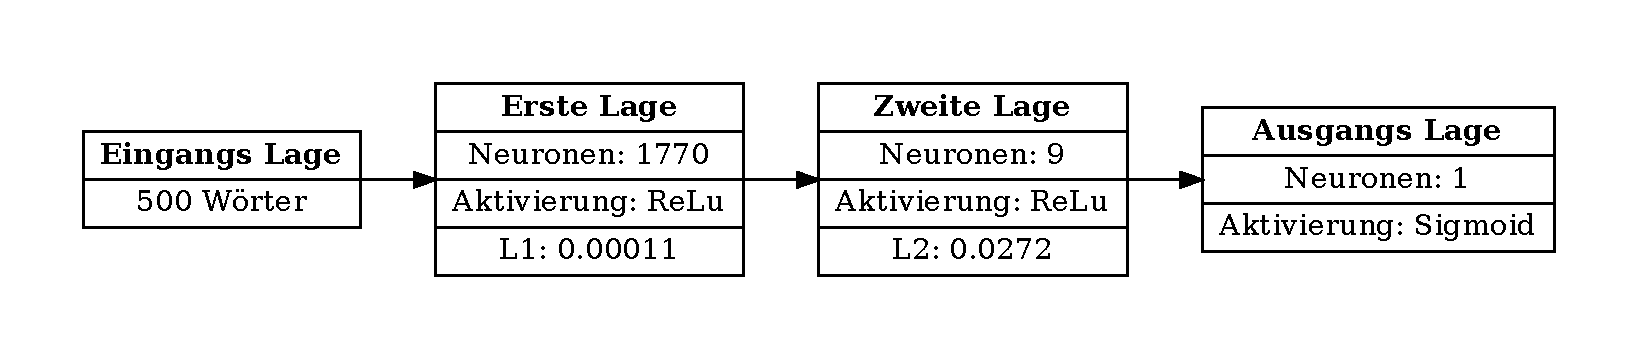
\includegraphics[width=0.8\textwidth]{pictures/modell_scheme.pdf}
    \caption{Schematische Darstellung des mit der \textsc{HYPERAS}-Bibliothek~\cite{hyperas} 
    optimierten DNN.}
    \label{fig:DNN_model}
\end{figure}





\chapter{Diskussion der Ergebnisse}
Die Verlustfunktion wird über $100$ Epochen bestimmt und für Trainings- und Validierungsdatensatz 
in Abbildung \ref{fig:history} dargestellt, wobei eine Batch-Size von $64$ verwendet wird. Nach ca.
$40$ Epochen bleibt der Validierungsverlust nahezu konstant, sodass weiteres Trainieren zu einer 
Überanpassung führen würde. Aus Abbildung \ref{fig:likelihood} ist ersichtlich, dass das Netz 
für den Trainingsdatensatz nur leicht bessere Vorhersagen trifft, sodass eine Überanpassung 
ausgeschlossen werden kann. Zusätzlich ist zu erkennen, dass die Verteilungen breit verteilt
sind, was die hohe \textit{cross-entropy} von $0.32$ erklärt. Es ergibt sich eine Genauigkeit 
von $0.9$ für Real News und $0.86$ für Fake News. Die in Abbildung \ref{fig:cnfsn__mtx}
dargestellte Confusion-Matrix deutet auf eine gute Performance des DNN auf dem Testdatensatz hin,
da vorallem die Hauptdiagonale ausgeprägt ist. Der hohe \textit{AUC} (area under curve)-Wert 
von $0.94$ der \textit{ROC} (receiver operating characteristic)-Kurve (Abbildung \ref{fig:roc})
deutet ebenfalls daraufhin, dass das DNN eine gute Performance hat.
\begin{figure}
    \centering
    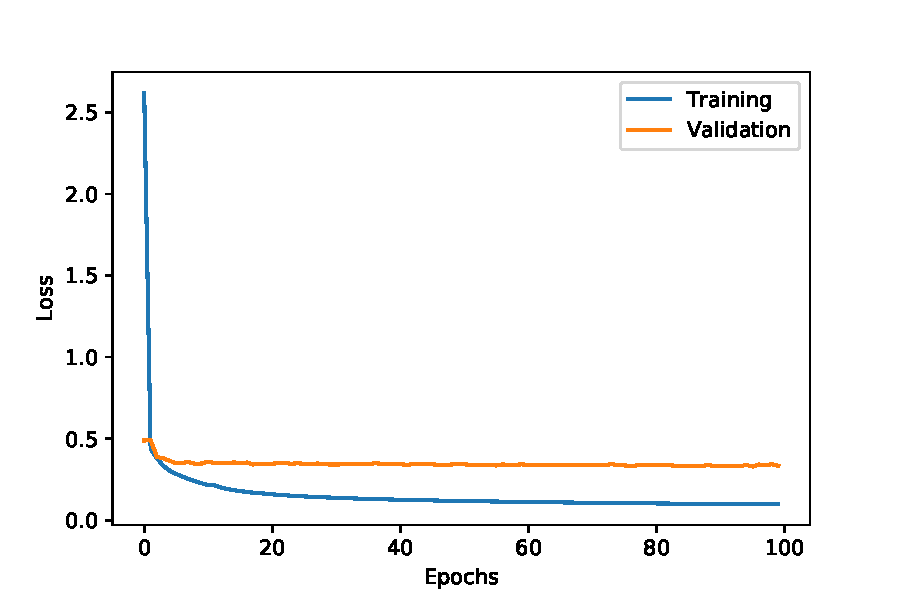
\includegraphics[width=0.8\textwidth]{pictures/history_bow_best.pdf}
    \caption{Es ist die Verlustfunktion, also \textit{cross-entropy} für Trainings- und 
    Validierungsdatensatz dargestellt. Es ist erkennbar, dass die jeweils als Real News 
    oder Fake News klassifizierten Texte, ähnliche Verteilungen besitzen.}
    \label{fig:history}
\end{figure}

\begin{figure}
    \centering
    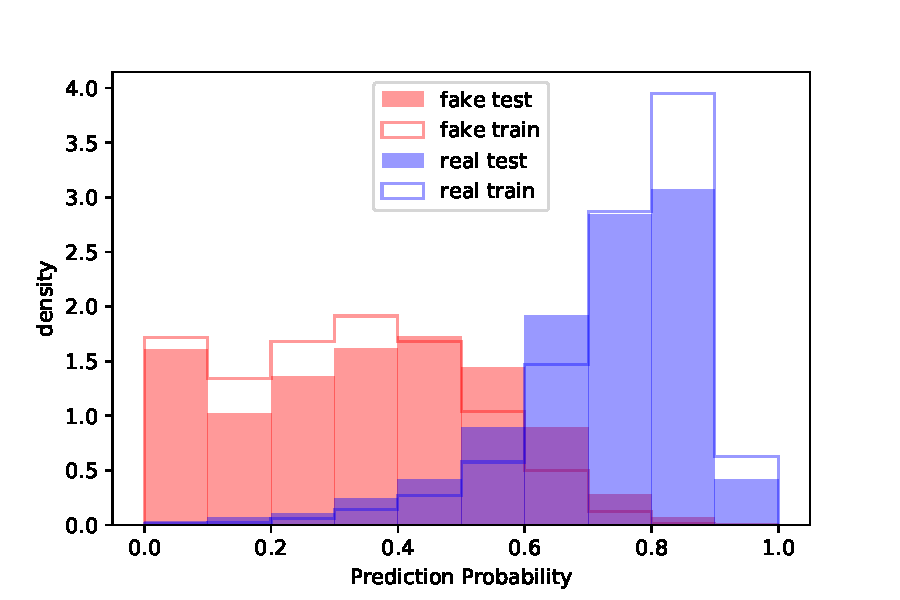
\includegraphics[width=0.8\textwidth]{pictures/prob_bow_best_nn.pdf}
    \caption{In dieser Abbildung ist die Likelihood für die verschiedenen Klassen für Trainingsdatensatz 
    und Testdatensatz dargestellt.}
    \label{fig:likelihood}
\end{figure}

\begin{figure}
    \centering
    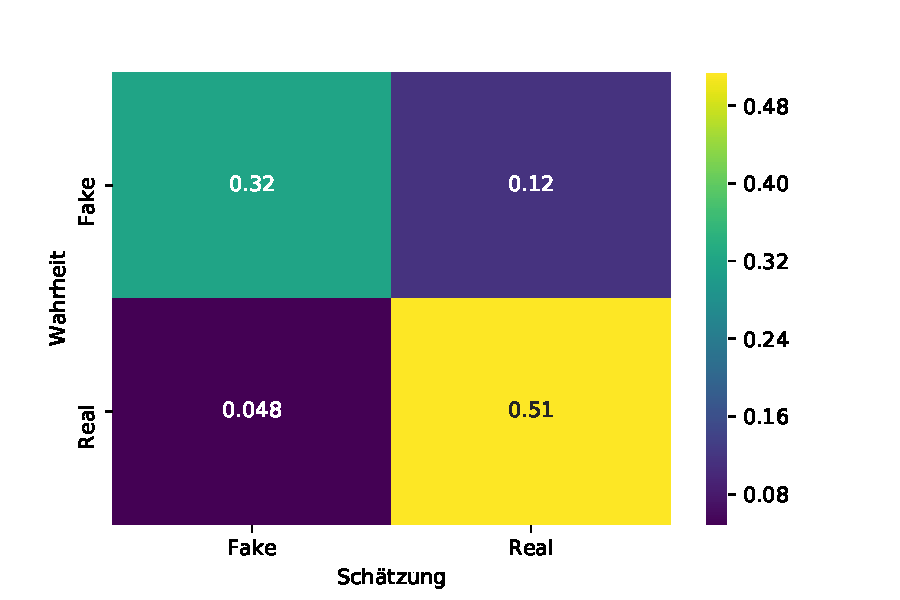
\includegraphics[width=0.8\textwidth]{pictures/cnfsn_mtx_bow_best_nn.pdf}
    \caption{Es ist die Confusion-Matrix des Testdatensatzes dargestellt. Es ist 
    zu erkennen, dass vorallem die Hauptdiagonale ausgeprägt ist, was für eine 
    gute Performance des DNN spricht.}
    \label{fig:cnfsn__mtx}
\end{figure}

Zur Interpretation der Vorhersagen des Netzes, werden die Beträge der Gewichte der ersten versteckten Lage,
die zu einem Wort gehören, aufsummiert. Unter der Annahme, dass ein hohes Gewicht einen 
hohen Einfluss auf die Vorhersage des Netzes hat, können die Wörter bestimmt werden,
die das Netz vorallem berücksichtigt. Die relativen Häufigkeiten der so bestimmten wichtigsten 
Wörter werden in einer Confusion-Matrix in Abbildung \ref{fig:cnfn_hist} dargestellt. An dieser 
Abbildung ist zu erkennen, dass die jeweils falsch klassifizierten Texte ähnliche Histogramme haben,
wie die richtig klassifizierten Texte, sodass es zu einer Verwechslung kommt. 

\begin{figure}
    \centering
    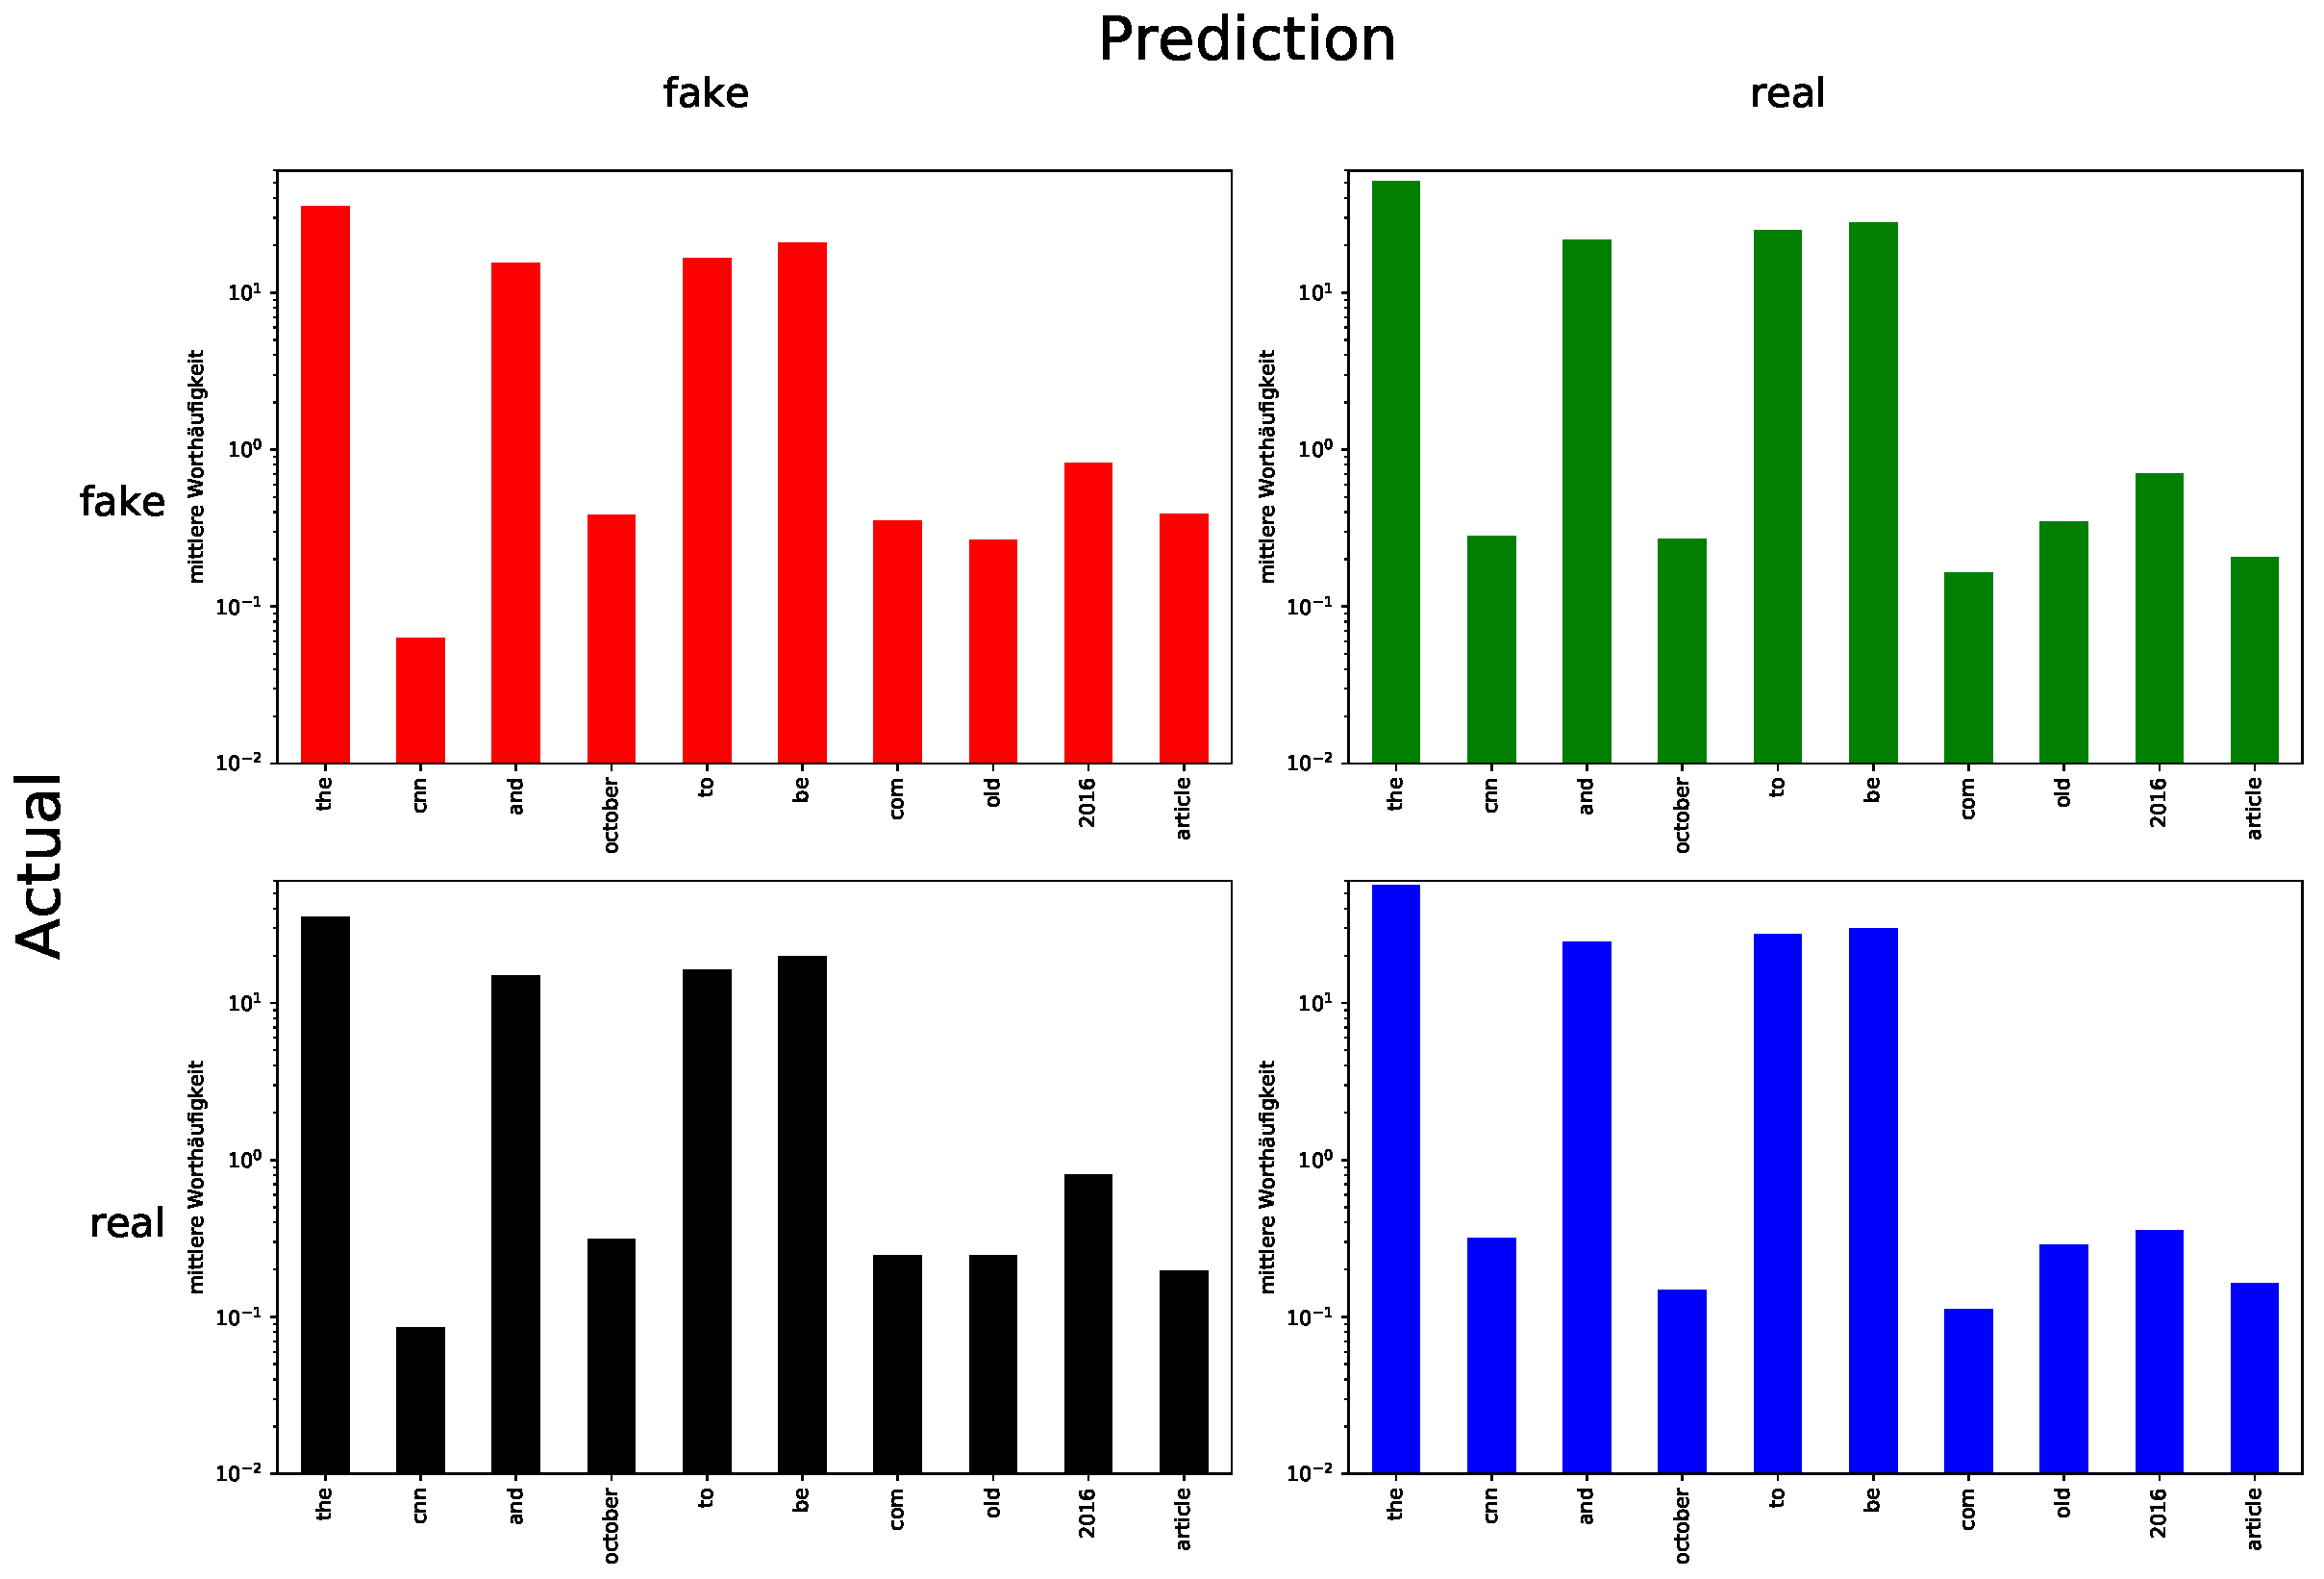
\includegraphics[width=0.8\textwidth]{pictures/cnfn_hist.pdf}
    \caption{Confusion Matrix mit relativer Häufigkeit der Wörter, die 
    im DNN stark gewichtet werden.}
    \label{fig:cnfn_hist}
\end{figure}

Beispielsweise ist das Wort \enquote{the} in den als Fake News klassifizierten Texten häufiger, als in den als 
Real News klassifizierten Texten. Es lässt sich daher vermuten, da es sich bei diesem Wort um 
ein Stoppwort handelt, sich daraus die ursprüngliche Textlänge abschätzen lässt, die im Mittel
für Real News länger ist, als für Fake News. Wichtig ist auch die Top-Level-Domain \enquote{com},
welche in den Fake News häufiger vorkommt. Dies liegt vermutlich daran, dass in den Fake News 
häufiger URL-Verlinkungen auftauchen, als in den Real News. Im Gegensatz dazu wird in Real News 
die Zeitung \enquote{CNN} häufiger erwähnt, da in diesen häufiger andere journalistische 
Zeitungen zitiert werden. Die Wichtigkeit von zeitlichen Angaben, wie \enquote{2016} und \enquote{october},
die in dem Zeitraum liegen, aus welchem die Daten stammen, lässt vermuten, dass das trainierte 
Netz sich nur für Vorhersagen aus diesem Zeitraum eignet.\\
Zum Schluss geht es um die Frage, ob die aufwendige Struktur eines DNN gerechtfertigt ist, oder 
ob es nicht möglich ist mit einem einfacheren Lösungsansatz ähnliche Ergebnisse zu erzielen. Es 
wird als Alternativmethode ein Random Forest verwendet, da dieser für Klassifizierungsaufgaben 
geeignet ist. Es wird der \textit{RandomForestClassifier} von \textsc{scikit-learn} verwendet.
Als Eingabedaten erhält dieser ebenfalls, die Bag-of-words Vektoren, besteht 
aus $100$ Entscheidungsbäumen mit maximaler Tiefe $10$ und als Einteilungskriterium die Entropie.\\
Obwohl die Hyperparameter des Random Forest nicht optimiert wurden, ergeben sich ähnliche 
Vorhersagegenauigkeiten, wie beim DNN. Die Vorhersagegenauigkeit für Real News beträgt 
$0.81$, ist also schlechter als die Vorhersagegenauikeit des DNN. Für Fake 
News ist die Genauigkeit mit $0.87$ sogar besser. Dies spiegelt sich auch in der 
\text{ROC}-Kurve (Abbildung \ref{fig:roc}) wider, die für sehr niedrigere Werte besser ist,
als die des DNN und schlechter für größere Werte. Der \textit{AUC}-Wert ist mit 
$0.92$ kleiner, als der des DNN.\\
\begin{figure}
    \centering
    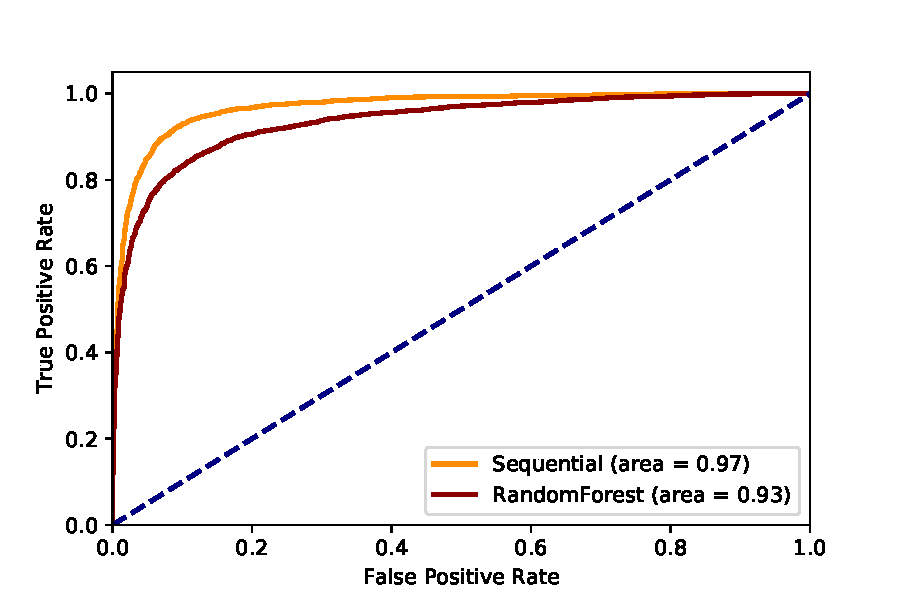
\includegraphics[width=0.8\textwidth]{pictures/roc_comparison.pdf}
    \caption{Hier ist die \text{ROC}-Kurve für das DNN und den Random Forest dargestellt.
    Beide Kurven haben einen hohen \textit{AUC}-Wert und eine nahezu rechteckige Form,
    was für eine gute Performance spricht.}
    \label{fig:roc}
\end{figure}



\chapter{Zusammenfassung und Ausblick}
Die eingangs gestellte Fragestellung, ob sich Fake News von Real News mittels 
Methoden des maschinellen Lernen unterscheiden lassen, kann zumindest eingeschränkt
auf den verwendeten Datensatz beantwortet werden. Die gute Perfomance des Netzes spricht 
dafür, dass es prinzipiell möglich ist einen Teil zu unterscheiden, es bleibt aber ein 
Rest, vorallem von als Real News klassifierten Fake News mit Anteil von $0.14$, bei 
denen die gegebenen Informationen nicht ausreichen, wie in Abbildung \ref{fig:cnfn_hist}
zu sehen ist. Eventuell könnten aktuellere Methoden, wie ein LSTM (Long-Short-Term-Memory)
oder Googles \textsc{Bert}(Bidirectional Encoder Representations from Transformers) bessere
Ergebnisse liefern. Erste Versuche in diese Richtung konnten dies jedoch nicht bestätigen.

Die begrenzte Verwendbarkeit dieses Datensatzes zur Klassifizierung zukünftiger Nachrichten  
werden vorallem durch die Wörter deutlich, die sich auf einen bestimmten Zeitraum beziehen.
Außerdem sind die Themen des Datensatzes auch inhaltlich durch die Themen des US-Wahlkampfes 
dominiert. Zur Verringerung des so begangenen systematischen Fehlers wird es nötig sein,
den Datensatz auf größere Zeiträume auszuweiten. Zusätzlich müsste die Liste der Quellen
stetig aktuell gehalten und manuell erweitert werden, um neue Quellen für Fake News 
nicht auszuschließen.

\appendix
% Hier beginnt der Anhang, nummeriert in lateinischen Buchstaben
%\input{content/a_anhang.tex}

\backmatter
\printbibliography

\end{document}
